\documentclass[a4paper,10pt]{article}
\usepackage[utf8]{inputenc}
\usepackage{amsmath}					%for advanced mathmematical formulas
\usepackage{graphicx}					%always use this package if you want to insert graphics into your report
\usepackage{fullpage}



\graphicspath{{./graphs/algorithm1/}{./graphs/algorithm2/}{./graphs/algorithm3/}{./graphs/*}}


% Title Page
\title{\Huge{One-Dimensional Line Search Methods Assignment}\\[7cm]Advanced Design 814\\[2cm]}

\author{\Large Andreas Joss\\[0.5cm]16450612}
\date{\today}

\begin{document}
\maketitle


\newpage
\section{Introduction}
This report briefly explains the  three different one-dimensional line search methods which are used for this assignment. Furthermore, the algorithms are implemented in code and the results thereof are shown and discussed. 

\section{Theory}
\subsection{Newton-Raphson Method}
The Newton-Raphson method can be derived from the Taylor Series expansion which is used to approximate functions. The Newton-Raphson method is described as:
 \begin{equation}\label{eq:1}
  x^{*} \approx x^{k+1} = x^{k} - \frac{f'(x^{k})}{f''(x^{k})}
 \end{equation}
\\[0.5cm]

where $x^{k+1}$ describes the next solution and $x^{k}$ describes the present solution.

\subsection{Newton-Raphson Method Modified}
The purpose of this modification is to ensure that a solution is found for the given problem function, for cases where the normal Newton-Raphson method would diverge. This modified method might require more iterations than the unmodified method, nevertheless convergence is more likely.
\\[0.5cm]
The modified Newton-Raphson method is described as:
 \begin{equation}\label{eq:2}
  x^{*} \approx x^{k+1} = x^{k} - \frac{f'(x^{k})}{\text{max}(f''(x^{k}),\epsilon)}
 \end{equation}
\\[0.1cm]

For the denominator of Equation \ref{eq:2}, the maximum value is selected being either the second derivative of the function at the current solution, or a value $\epsilon$ which is normally selected in the order of $\epsilon = 10^{-6}$. One problem arises in the unmodified Newton-Raphson method (Equation \ref{eq:1}) when the denominator is equal to zero or very close to zero. This causes the newly calculated solution $x^{k+1}$ to assume a value placed very far, or even infinitely far, from the previous solution $^{k}$, which as a result makes it very hard for the unmodified Newton-Raphson method to converge. The modification of the Newton-Raphson method ensures that the denominator is at least as large as $\epsilon$. The second problem of the unmodified method, is when the second derivative is found to be $f^{''}(x^{k}) < 0$. This means that the function is non-convex (concave) in that region and that the next solution will move closer to a non-converging region. The modified method, would then prevent the next solution to move into the aforementioned direction, by replacing $f^{''}(x^{k})$ with a small positive value $\epsilon$.

\subsection{Golden Section Method}
For this method to be useful, it is assumed that the objective function $f(x)$ has a minimum within an interval $[a,b]$ (which is selected from user experience), and that $f(x)$ is descending for $x < x^*$ and $f(x)$ is ascending for $x > x^*$. New points $x_{1}$ and $x_{2}$ are selected when certain criteria are met.

If $f(x_{2} > f(x_{1}$ then the new interval becomes $[a,x_{2}]$ with $b$ obtaining the new boundary value, otherwise the new interval will be $[x_{1},b]$ with $a$ obtaining the new boundary value. Thus, the interval is reduced until $x^{*}$ is reached within a prescribed accuracy. The ratio by which the interval is reduced, is determined by the golden ratio $r=0.618034$. The algorithm steps are explained in full by [1:37].

\section{Selecting the Appropriate Method}
\subsection{Newton-Raphson Methods}
From Equation \ref{eq:1} and \ref{eq:2} it is clear that first and second order derivative information of the objective test function is required to use the method. Depending on the problem at hand, it is up to the user to decide how practical this method is regarding the expensiveness to obtain this information. Even if the first and second order derivatives are obtained, the method could still struggle to deliver a global minimum due to its susceptibility to noise. For the modified Newton-Raphson method, values for $\epsilon$ can be chosen experimentally for specific problems. If the method still diverges, then a larger $\epsilon$ value could be selected.

\subsection{Golden Section Method}
For this method, only zero order information is required from the objective test function. This is useful when the first and second order derivative information is hard and expensive to obtain, but zero order information is more accessible. This method is consequently much less susceptible to noise.

\section{Example Functions}
Example functions are used to evaluate the effectiveness of each algorithm and briefly compare the algorithm results with each other. Each graph displays several parameters for the particular optimization at hand as well as the solution that is found. Each test function has its own specified boundaries and also the tolerance of the accuracy of the desired solution. The following test functions are used:
\\[0.5cm]
(i) minimize $F(\lambda) = \lambda^{2} + 2e^{-\lambda} \text{ over } [0,2] \text{ with } \epsilon = 0.01$
\\[0.5cm]
(ii) maximize $F(\lambda) = \lambda \text{cos} \lambda \text{ over } [0,\frac{\pi}{2}] \text{ with } \epsilon = 0.001$
\\[0.5cm]
(iii) minimize $F(\lambda) = 4(\lambda - 7) / (\lambda^{2} + \lambda - 2) \text{ over } [-1.9,0.9] \text{ with }$ by performing no more than 10 function iterations.
\\[0.5cm]
(i) minimize $F(\lambda) = \lambda^{4} + -20\lambda^{3} + 0.1\lambda \text{ over } [0,20] \text{ with } \epsilon = 10^{-5}$

\section{Results}
The algorithm are programmed in the Python language, due to future work which will also require extensive Python scripting. The Matplotlib library is used to display the results in a neat and informative manner. In each case the green dot indicates the solution that is found (if any) by the algorithm.

\newpage
\subsection{Newton-Raphson Method}
\begin{figure}[h]
\centering
 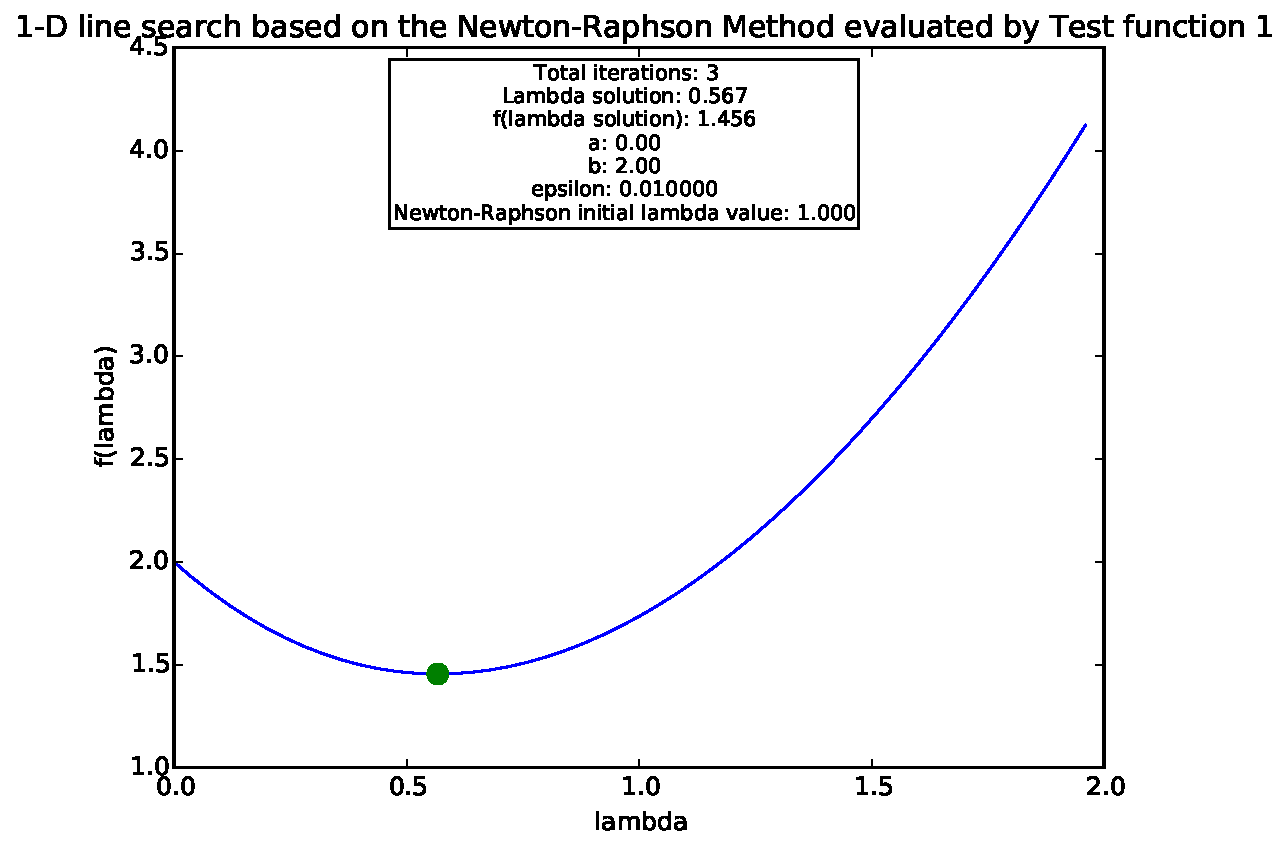
\includegraphics[scale=0.55]{./graphs/algorithm1/x_in_middel/testFunction1.pdf} 
 \caption{The Newton-Raphson Method evaluated by first example function}
 \label{fig:alg1test1}
\end{figure}

\begin{figure}[h]
\centering
 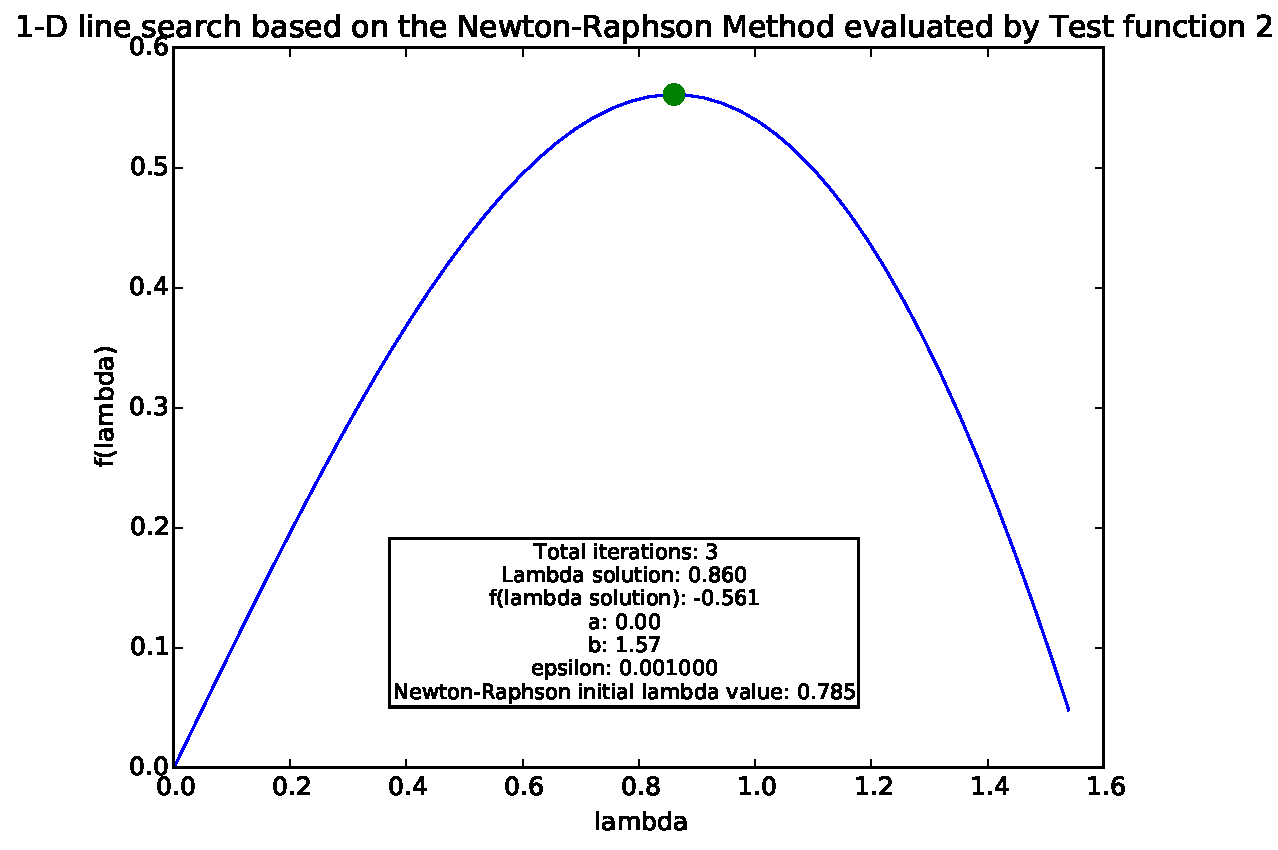
\includegraphics[scale=0.55]{./graphs/algorithm1/x_in_middel/testFunction2.pdf} 
 \caption{The Newton-Raphson Method evaluated by second example function}
 \label{fig:alg1test2}
\end{figure}

Figure \ref{fig:alg1test1} and Figure \ref{fig:alg1test2} show that this algorithm manages to successfully converge near or on the optimal point. Note for both test functions, only three iterations are required.

\newpage
\begin{figure}[h]
\centering
 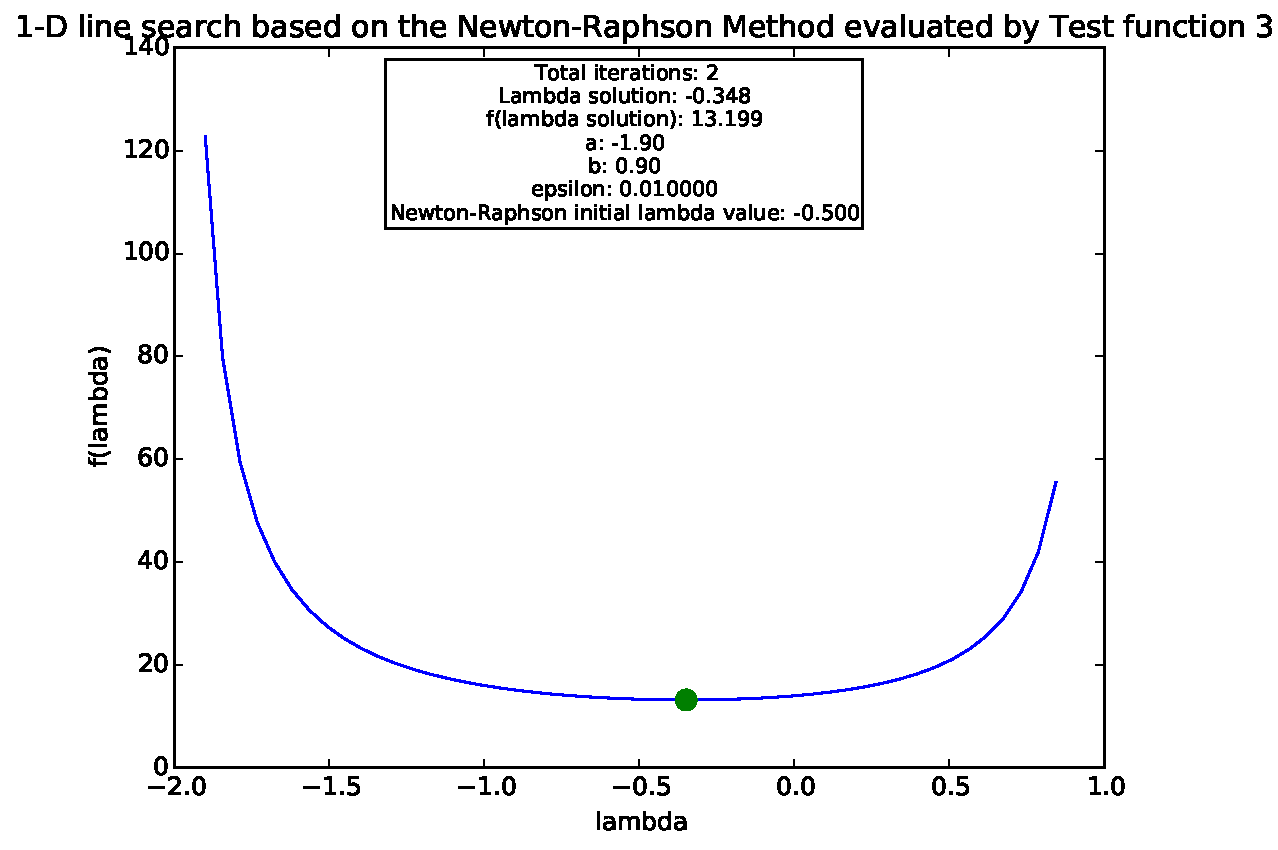
\includegraphics[scale=0.55]{./graphs/algorithm1/x_in_middel/testFunction3.pdf} 
 \caption{The Newton-Raphson Method evaluated by third example function}
 \label{fig:alg1test3}
\end{figure}

\begin{figure}[h]
\centering
 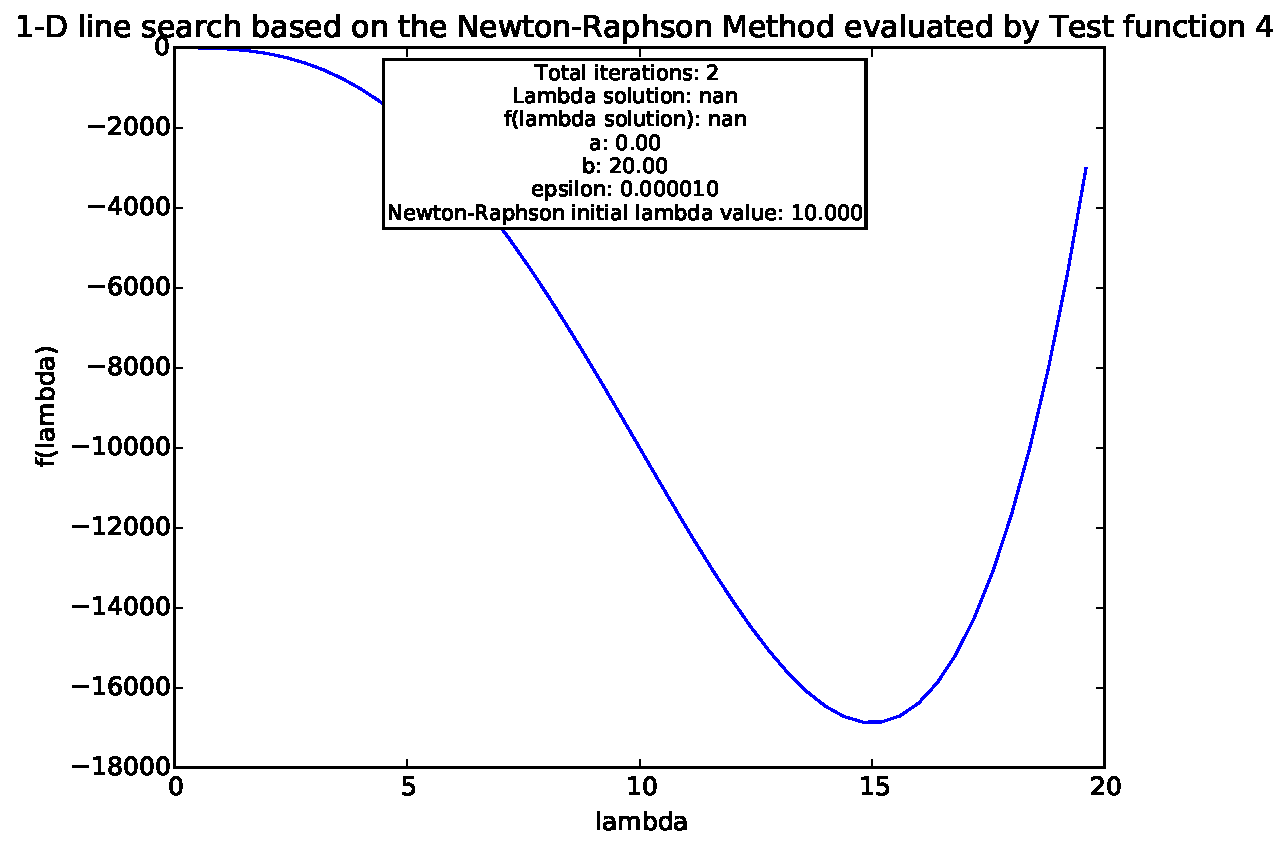
\includegraphics[scale=0.55]{./graphs/algorithm1/x_in_middel/testFunction4.pdf} 
 \caption{The Newton-Raphson Method evaluated by fourth example function}
 \label{fig:alg1test4}
\end{figure}

Figure \ref{fig:alg1test3} indicates that this algorithm manages to successfully converge near or on the optimal point. Note that only two iterations are required to adhere to the tolerance value. From Figure \ref{fig:alg1test4}, it is clear that the algorithm did not converge to a solution. This is due to the fact that the initial starting solution is not chosen adequately for this particular problem. 

\newpage
\begin{figure}[h]
\centering
 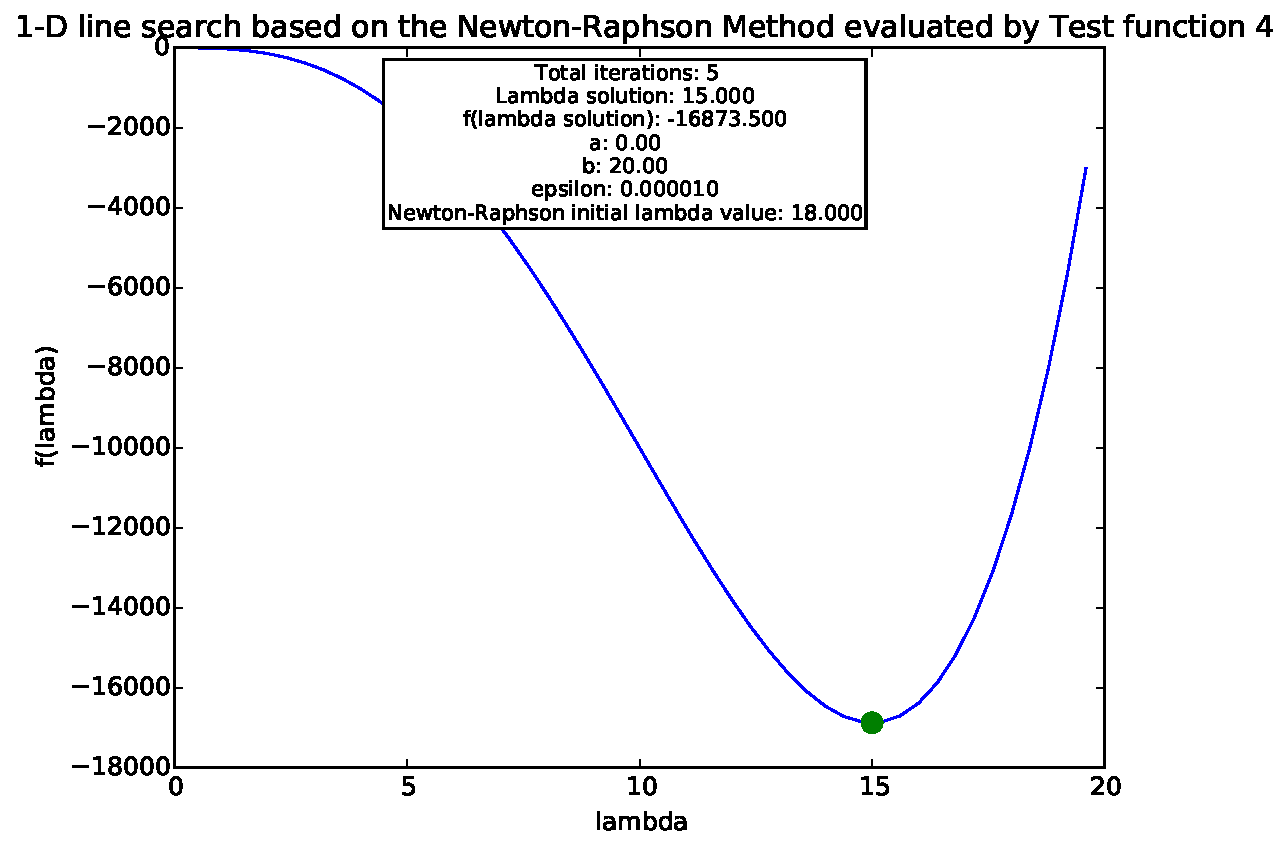
\includegraphics[scale=0.55]{./graphs/algorithm1/x90percentofb/testFunction4.pdf} 
 \caption{1-D line search based on the Newton-Raphson Method evaluated by fourth example function, with a new starting solution selected}
 \label{fig:alg1test4B}
\end{figure}

This time, from Figure \ref{fig:alg1test4B}, it is visible that the algorithm successfully converged to a solution. This is because a different starting estimated solution is assumed compared to the estimated starting solution of Figure \ref{fig:alg1test4}. This is indicated on the figures by ``Newton-Raphson initial lambda value: 10.0'' and ``Newton-Raphson initial lambda value: 18.0'' respectively.

\newpage
\subsection{Modification of the Newton-Raphson Method}
\begin{figure}[h]
\centering
 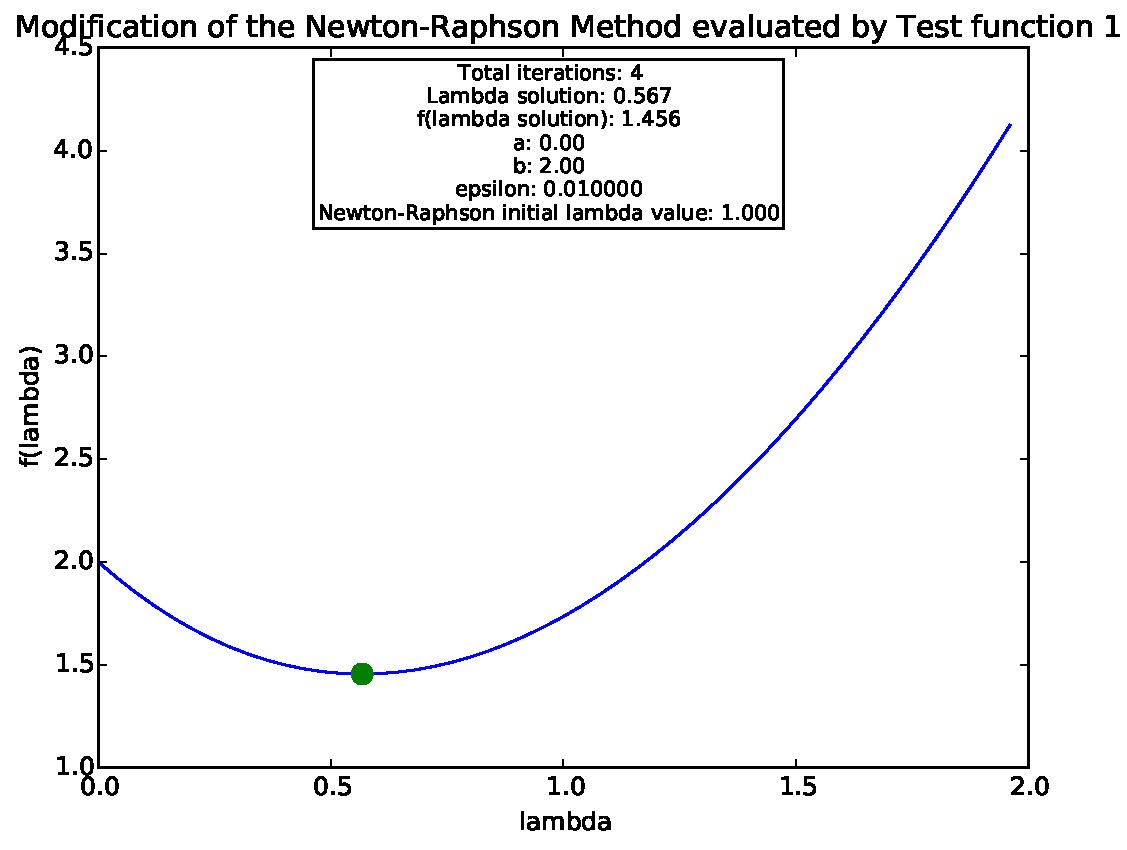
\includegraphics[scale=0.55]{./graphs/algorithm2/x_in_middel/testFunction1.pdf} 
 \caption{Modification of the Newton-Raphson evaluated by first example function}
 \label{fig:alg2test1}
\end{figure}

\begin{figure}[h]
\centering
 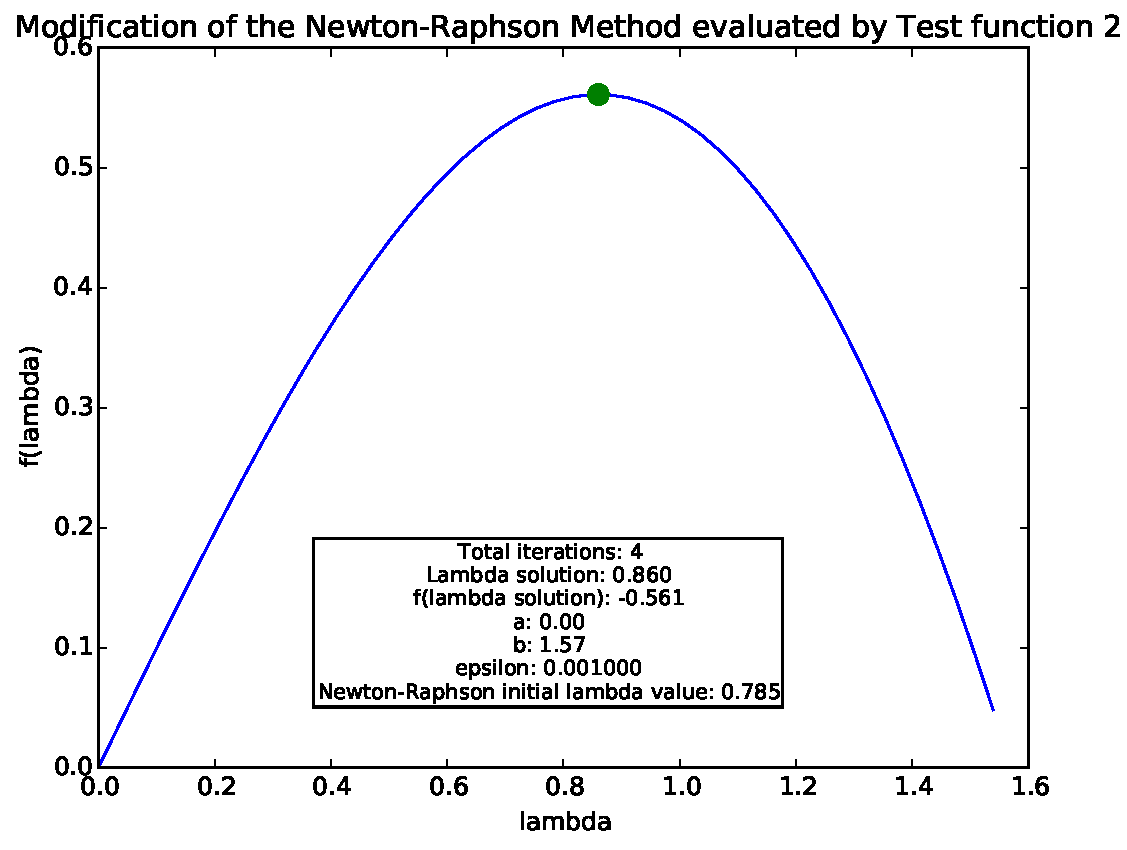
\includegraphics[scale=0.55]{./graphs/algorithm2/x_in_middel/testFunction2.pdf} 
 \caption{Modification of the Newton-Raphson evaluated by second example function}
 \label{fig:alg2test2}
\end{figure}

Figure \ref{fig:alg2test1} and Figure \ref{fig:alg2test2} show that this algorithm manages to successfully converge near or on the optimal point. Note that a slight increase in number of iterations are required, compared to the unmodified Newton-Raphson method's results shown by Figure \ref{fig:alg1test1} and Figure \ref{fig:alg1test2}.

\newpage
\begin{figure}[h]
\centering
 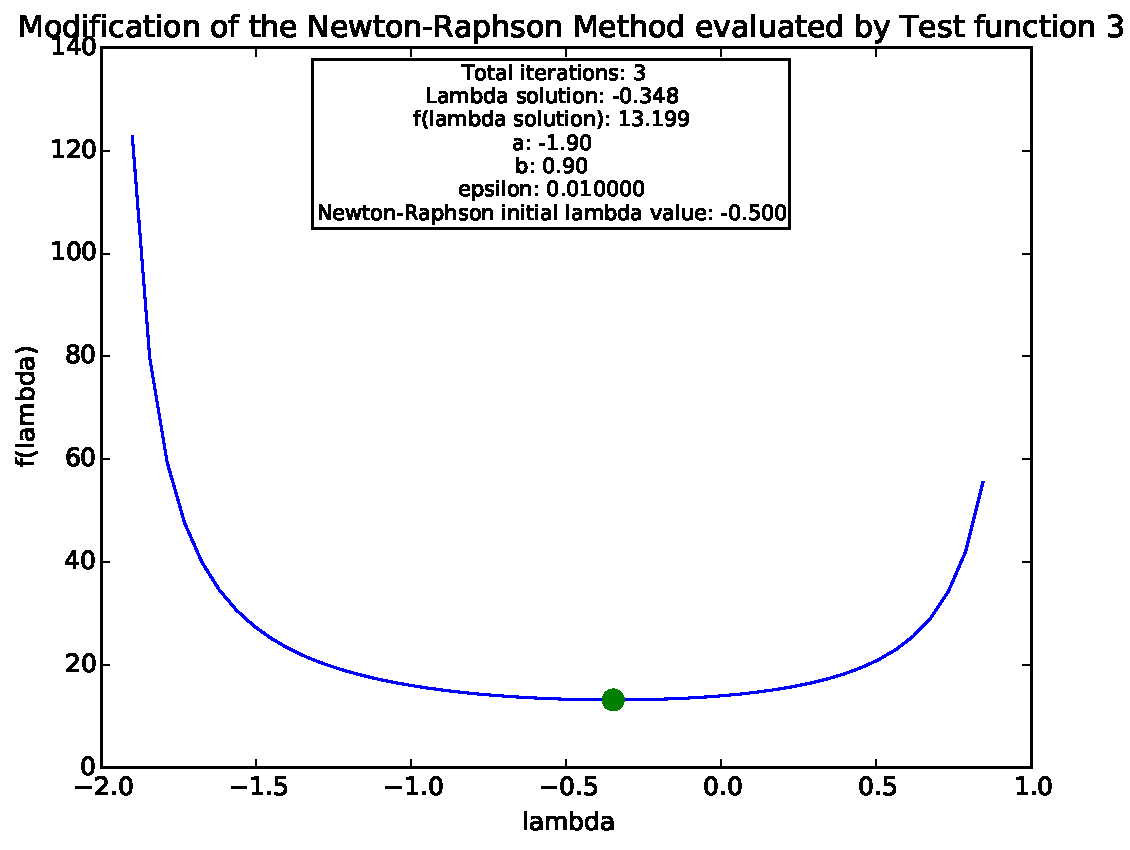
\includegraphics[scale=0.55]{./graphs/algorithm2/x_in_middel/testFunction3.pdf} 
 \caption{Modification of the Newton-Raphson evaluated by third example function}
 \label{fig:alg2test3}
\end{figure}

\begin{figure}[h]
\centering
 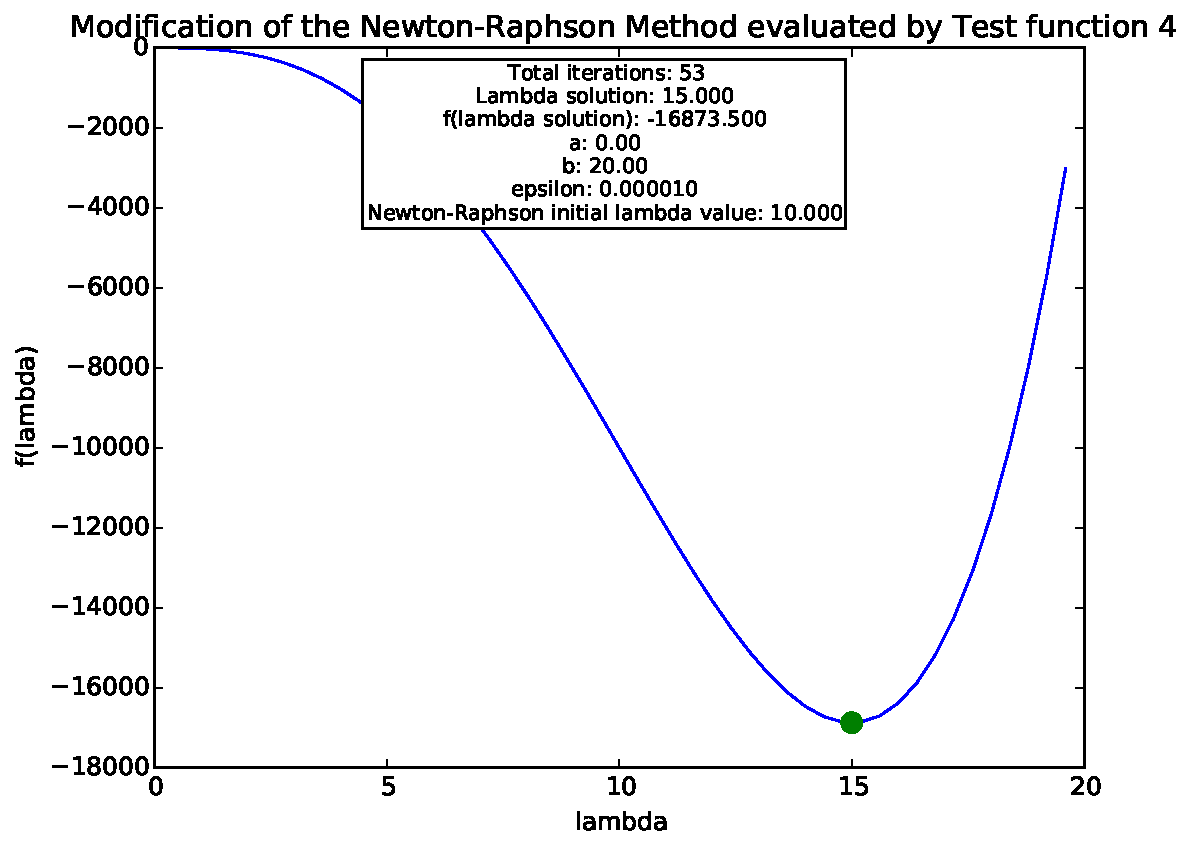
\includegraphics[scale=0.55]{./graphs/algorithm2/x_in_middel/testFunction4.pdf} 
 \caption{Modification of the Newton-Raphson evaluated by fourth example function}
 \label{fig:alg2test4}
\end{figure}

Figure \ref{fig:alg2test3} indicates that this algorithm manages to successfully converge. Notice that once again a slight increase of iterations (from 2 to 3) are needed to solve the third test function, as compared to the unmodified Newton-Raphson method shown in Figure \ref{fig:alg1test3}. Interestingly, Figure \ref{fig:alg2test4} converges with the same starting solution assumed by Figure \ref{fig:alg1test4} ; ``Newton-Raphson initial lambda value: 10.0''. This is expected, as the modification of the Newton-Raphson method will more likely converge than the unmodified Newton-Raphson method, even if much more iterations are required. The number of iterations required are 53, compared to Figure \ref{fig:alg1test4} where the algorithm diverged outside the boundaries within two iterations. Additionally, it is also not needed to choose a different start solution as was required by the test shown in Figure \ref{fig:alg1test4B}. 

\newpage
\subsection{Golden Section Method}
\begin{figure}[h]
\centering
 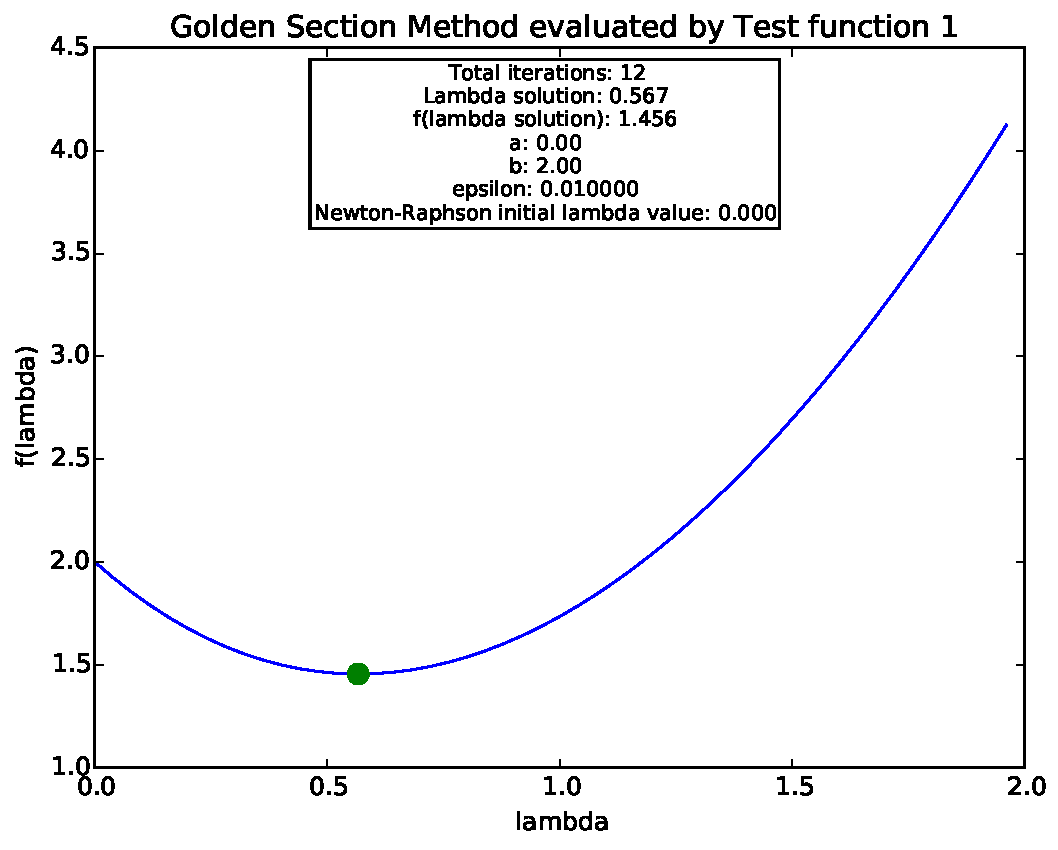
\includegraphics[scale=0.55]{./graphs/algorithm3/testFunction1.pdf} 
 \caption{Golden Section Method evaluated by first example function}
 \label{fig:alg3test1}
\end{figure}

\begin{figure}[h]
\centering
 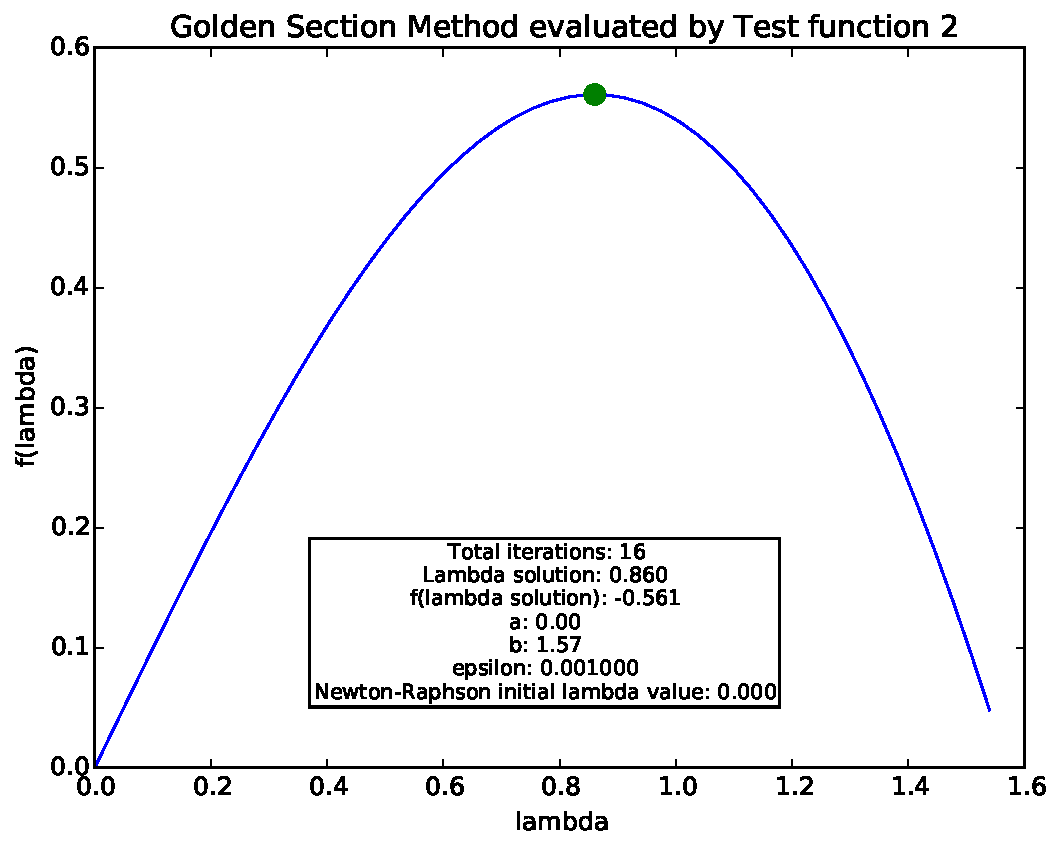
\includegraphics[scale=0.55]{./graphs/algorithm3/testFunction2.pdf} 
 \caption{Golden Section Method evaluated by second example function}
 \label{fig:alg3test2}
\end{figure}

Figure \ref{fig:alg3test1} and Figure \ref{fig:alg3test2} show that this algorithm manages to successfully converge near or on the optimal point. Note that much more iterations are required to achieve the equal accuracy of solutions as indicated by Figure \ref{fig:alg1test1} and Figure \ref{fig:alg1test2}.

\newpage
\begin{figure}[h]
\centering
 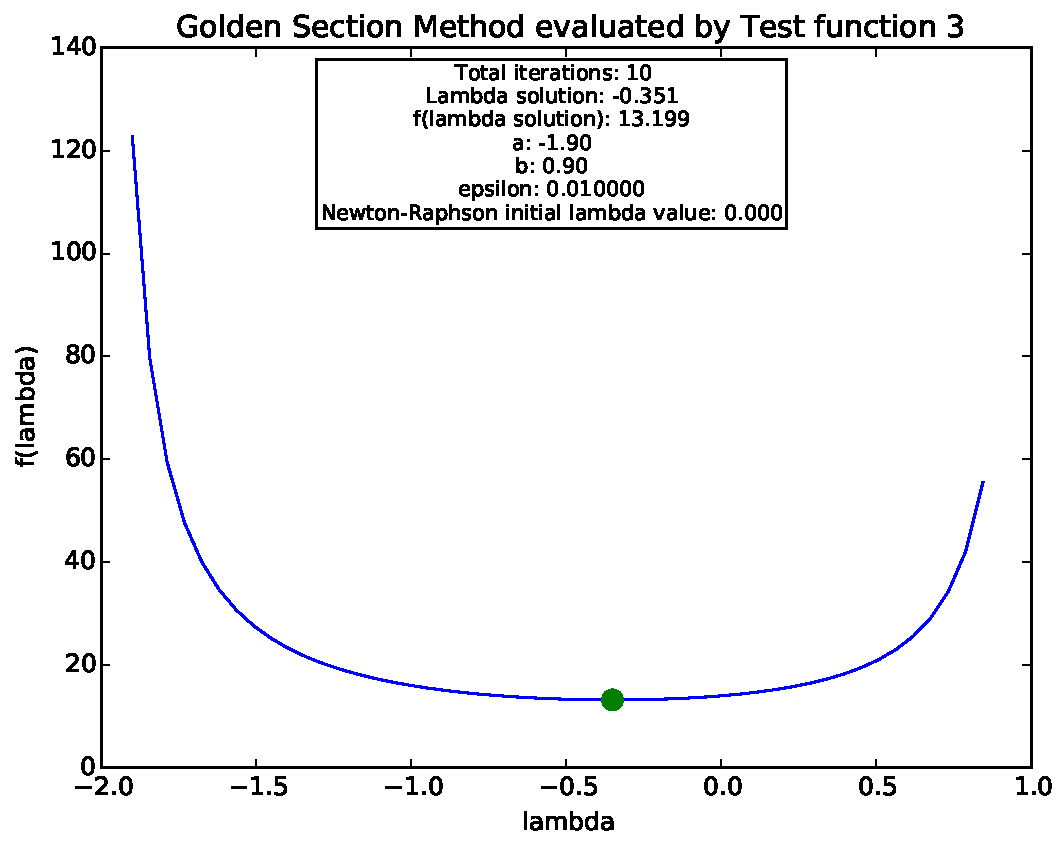
\includegraphics[scale=0.55]{./graphs/algorithm3/testFunction3.pdf} 
 \caption{Golden Section Method evaluated by third example function}
 \label{fig:alg3test3}
\end{figure}

\begin{figure}[h]
\centering
 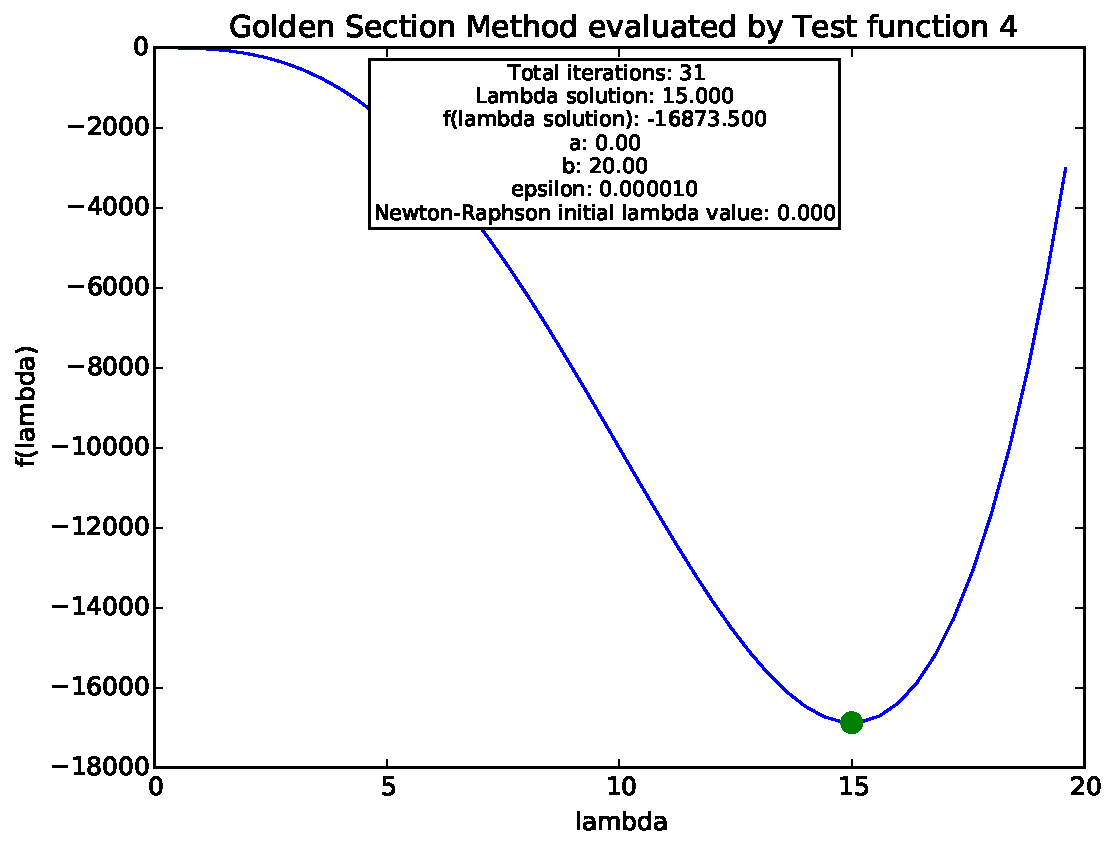
\includegraphics[scale=0.55]{./graphs/algorithm3/testFunction4.pdf} 
 \caption{Golden Section Method evaluated by fourth example function}
 \label{fig:alg3test4}
\end{figure}

Figure \ref{fig:alg3test3} indicates that this algorithm manages to successfully converge near or on the optimal point. It is also shown that the number of iterations are limited to 10 for the third test function. From Figure \ref{fig:alg3test4}, it is clear that the algorithm did converge to a solution. Notice that 31 iterations are required to obtain the solution, as compared to Figure \ref{fig:alg1test4B} where only 5 iterations are required (given the starting point chosen for that example).

\newpage
\section{Conclusion}
The Newton-Raphson method proved to converge very quickly to the correct solution if the test function is convex at the location of the starting position that is chosen. If divergence occurs, it is possible to select a different starting position and achieve convergence within a relative low number of iterations.\\[0.4cm]
The modification of the Newton-Raphson method shows that it takes slightly longer to converge to the correct solution as compared to the unmodified method. However, in the case where the unmodified Newton-Raphson method would diverge, the modified method would at least find the solution even if much more iterations are required (without needing to choose a different starting position).\\[0.4cm]
The Golden Section method proved to be a very useful tool when first and second order derivative information is not available, and only zero order function values can be obtained. From the test functions that are used in this report, it seems that the Golden Section method is also rather rugged in the sense of converging to the global optimum. It is noted that the Golden Section method in general requires more iterations to obtain the solution, however that this does conclude for it to be a slower method than the Newton-Raphson method. The solve speed would also depend on the specific problem at hand and the time-expensiveness of obtaining zero, first and second order derivative information.

\section{Bibliography}
1. Snyman J. Practical Mathmematical Optimization. Technical report, Department of Mechanical and Aeronautical Engineering University of Pretoria, Pretoria, South Africa, 2005. 

\end{document}   